\chapter{Literature review} \label{chap:sota}

\section*{}

% Neste capítulo é descrito o estado da arte e são
%apresentados trabalhos relacionados para mostrar o que existe no
%mesmo domínio e quais os problemas em aberto.
%Deve deixar claro que existe uma oportunidade de desenvolvimento que
%cobre alguma falha concreta .

%O capítulo deve também efetuar uma revisão tecnológica às principais
%ferramentas utilizáveis no âmbito do projeto, justificando futuras
%escolhas.

\section{Introduction}

%Neste capítulo é ilustrada a utilização de macros \LaTeX\ para definir
%entradas no índice remissivo e são feitas diversas referências
%bibliográficas, usando-se texto de um artigo apresentado na %Conferência 
% XATA2006~\cite{kn:MVL06-xata}.

% Nos últimos tempos têm surgido diversas soluções, apresentadas por
%empresas do sector Automação de Sistemas para a disponibilização de
%sistemas \scadadms{} na \textit{Web}.

\section{E-commerce background}

\subsection{Customer life cycle}

\begin{figure}[t]
  \begin{center}
    \leavevmode
    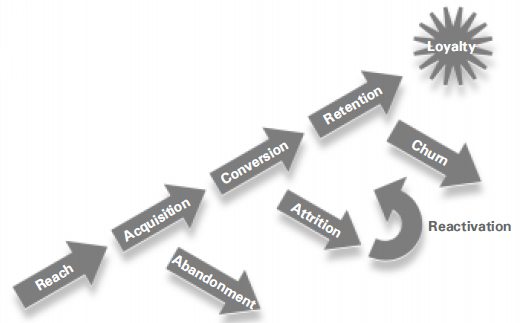
\includegraphics[width=0.86\textwidth]{lifecycle}
    \caption{Arquitectura da Solução Proposta}
    \label{fig:lifecycle}
  \end{center}
\end{figure}

Reach -> Acquisition/Abandonment -> Conversion/Attrition -> Retention / Churn -> Loyalty

\subsection{E-commerce metrics}

\cite{Sterne2000}

\subsection{Influencing user behaviour}

-> influenciar behaviour em vez de recom

\subsubsection{Recommendation engines}

\cite{Adomavicius2005}

\section{System Simulation}

\subsection{Agent Based Simulation (ABS)}

\cite{Siebers2010}

\subsection{Discrete Event Simulation (DES)}

\cite{Siebers2010}

\subsection{System Dynamics (SD)}

\cite{Siebers2010}

\section{Probabilistic Models}

Probabilistic or statistical models represent explicit assumptions about a problem domain, in the form of a model. This model usually encompasses random variables, in the form of probability distributions, and the relation and dependence between the variables. \cite{Winn2013}

In the following sections we describe a common way to represent probabilistic models, probabilistic graphical models (PGM) or, simply, graphical models.


\subsection{Probabilistic Graphical Models}



\begin{figure}[t]
	\begin{center}
		\leavevmodesharex
		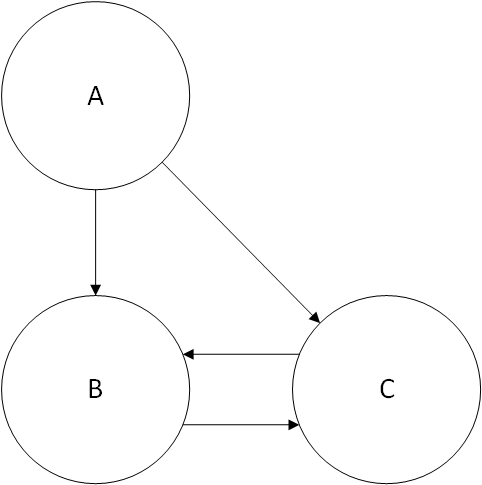
\includegraphics[width=0.36\textwidth]{pgm}
		\caption{Example of a PGM}
		\label{fig:pgm}
	\end{center}
\end{figure}

\ref{fig:pgm}

\subsection{Bayesian Networks}

\subsection{Markov Random Fields}

\subsection{Hidden Markov Models}

\cite{Rabiner1989}

\section{Summary}

No final do capítulo deverá ser apresentado um resumo com as 
principais conclusões que se podem tirar. 
